\documentclass[10pt,letterpaper,twocolumn]{article}
\usepackage[letterpaper,left=0.75in,right=0.75in,top=0.75in,bottom=1in,columnsep=24pt,headheight=12pt,headsep=22pt]{geometry}
\usepackage[T1]{fontenc}
\usepackage{mathptmx}
\renewcommand{\ttdefault}{pcr}
\usepackage{amsmath,booktabs,graphicx,array}
\usepackage{pgfplots}
\pgfplotsset{compat=1.18}
\usepgfplotslibrary{groupplots}
\usetikzlibrary{arrows.meta,positioning,calc}
\definecolor{figblue}{HTML}{0072B2}
\definecolor{figred}{HTML}{D55E00}
\definecolor{figgray}{HTML}{4D4D4D}
\usepackage[font=small,labelfont=bf,labelsep=colon]{caption}
\usepackage[hidelinks]{hyperref}
% Generated by generate_results.py; edit accepted source data only through review.
\newcommand{\PrimaryRows}{
4 & FCFS & 103.970 & 8,856 & 13.072 & 0.034 \\
4 & RR & 79.047 & 6,782 & 20.519 & 0.049 \\
4 & Main & 110.090 & 9,011 & 10.496 & 0.040 \\
8 & FCFS & 208.438 & 17,677 & 8.715 & 0.104 \\
8 & RR & 158.261 & 13,556 & 19.670 & 0.104 \\
8 & Main & 219.345 & 17,932 & 5.714 & 0.104 \\
16 & FCFS & 416.886 & 35,318 & 3.892 & 0.104 \\
16 & RR & 316.614 & 27,102 & 18.694 & 0.095 \\
16 & Main & 437.623 & 35,773 & 1.158 & 0.084 \\
}
\newcommand{\OverheadRows}{
4 & 5.89 & 39.27 & 1132.0 & 263.0 & 7144.0 \\
8 & 5.23 & 38.60 & 2767.6 & 512.9 & 13596.4 \\
16 & 4.97 & 38.22 & 6038.5 & 1268.7 & 26673.2 \\
}
\newcommand{\AreaFCFS}{(4,103.970058316) (8,208.437730604) (16,416.886135213)}
\newcommand{\PolicyFCFS}{(4,1.131957400) (8,2.767628100) (16,6.038461400)}
\newcommand{\SetupFCFS}{(4,13.071612000) (8,8.714740000) (16,3.891612000)}
\newcommand{\AreaRR}{(4,79.047172316) (8,158.260808962) (16,316.614126327)}
\newcommand{\PolicyRR}{(4,0.263039000) (8,0.512862600) (16,1.268686900)}
\newcommand{\SetupRR}{(4,20.519341000) (8,19.669725000) (16,18.694050000)}
\newcommand{\AreaMain}{(4,110.089845892) (8,219.344574607) (16,437.622506788)}
\newcommand{\PolicyMain}{(4,7.143987900) (8,13.596449900) (16,26.673175400)}
\newcommand{\SetupMain}{(4,10.496409000) (8,5.713676000) (16,1.158148000)}
\newcommand{\ColdPowerRows}{
4 & FCFS & 3.397 & 3.399 & 3.398 & 116.9 \\
4 & RR & 2.600 & 2.602 & 2.600 & 89.5 \\
4 & Main & 3.500 & 3.501 & 3.500 & 120.5 \\
8 & FCFS & 6.728 & 6.729 & 6.725 & 222.4 \\
8 & RR & 5.175 & 5.175 & 5.173 & 171.0 \\
8 & Main & 6.924 & 6.924 & 6.920 & 228.9 \\
16 & FCFS & 13.4 & 13.4 & 13.4 & 441 \\
16 & RR & 10.3 & 10.3 & 10.3 & 339 \\
16 & Main & 13.8 & 13.8 & 13.8 & 454 \\
}
\newcommand{\ColdMeanFCFS}{(4,3.398) (8,6.727) (16,13.400)}
\newcommand{\ColdSeedsFCFS}{(3.76,3.397) (4.00,3.399) (4.24,3.398) (7.76,6.728) (8.00,6.729) (8.24,6.725) (15.76,13.400) (16.00,13.400) (16.24,13.400)}
\newcommand{\ColdMeanRR}{(4,2.601) (8,5.174) (16,10.300)}
\newcommand{\ColdSeedsRR}{(3.76,2.600) (4.00,2.602) (4.24,2.600) (7.76,5.175) (8.00,5.175) (8.24,5.173) (15.76,10.300) (16.00,10.300) (16.24,10.300)}
\newcommand{\ColdMeanMain}{(4,3.500) (8,6.923) (16,13.800)}
\newcommand{\ColdSeedsMain}{(3.76,3.500) (4.00,3.501) (4.24,3.500) (7.76,6.924) (8.00,6.924) (8.24,6.920) (15.76,13.800) (16.00,13.800) (16.24,13.800)}
\newcommand{\BoundaryRows}{
FCFS & 1.309 & 0.01912 & 2.056 & 3.383 & 153.5 \\
RR & 1.001 & 0.01453 & 1.570 & 2.586 & 117.3 \\
Main & 1.334 & 0.02043 & 2.141 & 3.495 & 158.6 \\
}
\newcommand{\BoundaryInternal}{(1,1.309) (2,1.001) (3,1.334)}
\newcommand{\BoundarySwitching}{(1,0.01912) (2,0.01453) (3,0.02043)}
\newcommand{\BoundaryLeakage}{(1,2.056) (2,1.570) (3,2.141)}
\newcommand{\SupplementRows}{
Total area (library units) & 110089.846 & 110058.332 \\
Policy subtree area & 7143.988 & 7120.861 \\
Flip-flop cells & 9,011 & 9,011 \\
Setup slack (ns) & 10.496409 & 10.547482 \\
Hold slack (ns) & 0.039940 & 0.039940 \\
Constant-disabled checks & 68 & 68 \\
}

% Deterministic output of generate_hog_sparse_results.py; accepted five-seed RTL data.
\pgfplotstableread[row sep=\\]{
x y lo hi\\
1 16.3921250103 0.0221335354 0.0260335575\\
2 23.2989166667 0.1305833333 0.1006666667\\
}\HSMeanFCFS
\pgfplotstableread[row sep=\\]{
x y lo hi\\
1 18.2000000000 0.2000000000 0.8000000000\\
2 33.8000000000 2.8000000000 2.2000000000\\
}\HSPtailFCFS
\pgfplotstableread[row sep=\\]{
x y lo hi\\
1 0.9767280000 0.0007780000 0.0007120000\\
2 0.9765761719 0.0000136719 0.0000546875\\
}\HSHeavyFCFS
\pgfplotstableread[row sep=\\]{
x y lo hi\\
1 5.5979345050 0.0812970269 0.0879316890\\
2 9.1693333333 0.2160000000 0.1040000000\\
}\HSMeanRR
\pgfplotstableread[row sep=\\]{
x y lo hi\\
1 11.0000000000 0.0000000000 0.0000000000\\
2 17.2000000000 0.2000000000 0.8000000000\\
}\HSPtailRR
\pgfplotstableread[row sep=\\]{
x y lo hi\\
1 0.9767260000 0.0007760000 0.0007040000\\
2 0.9765644531 0.0000019531 0.0000078125\\
}\HSHeavyRR
\pgfplotstableread[row sep=\\]{
x y lo hi\\
1 5.5295627820 0.1048692619 0.0851004746\\
2 9.3243333333 0.2976666667 0.1590000000\\
}\HSMeanMain
\pgfplotstableread[row sep=\\]{
x y lo hi\\
1 10.0000000000 0.0000000000 0.0000000000\\
2 20.8000000000 3.8000000000 3.2000000000\\
}\HSPtailMain
\pgfplotstableread[row sep=\\]{
x y lo hi\\
1 0.9767240000 0.0007740000 0.0007060000\\
2 0.9765644531 0.0000019531 0.0000078125\\
}\HSHeavyMain
\newcommand{\HSReductionAFCFS}{45.03}
\newcommand{\HSReductionARR}{9.09}
\newcommand{\HSReductionBFCFS}{38.64}
\newcommand{\HSReductionBRR}{-20.78}
\pgfplotstableread[row sep=\\]{
x y lo hi\\
1 45.0292397661 0.5847953216 2.3391812865\\
2 9.0909090909 0.0000000000 0.0000000000\\
3 38.6401012018 9.2283364959 6.5211891208\\
4 -20.7843137255 20.3921568627 20.7843137255\\
}\HSPaired
\newcommand{\HSPairedSeeds}{(0.88,44.4444444444) (0.94,44.4444444444) (1.00,44.4444444444) (1.06,47.3684210526) (1.12,44.4444444444) (1.88,9.0909090909) (1.94,9.0909090909) (2.00,9.0909090909) (2.06,9.0909090909) (2.12,9.0909090909) (2.88,29.4117647059) (2.94,44.1176470588) (3.00,33.3333333333) (3.06,45.1612903226) (3.12,41.1764705882) (3.88,-41.1764705882) (3.94,-11.7647058824) (4.00,-33.3333333333) (4.06,0.0000000000) (4.12,-17.6470588235)}
\newcommand{\HSMeanAFCFS}{16.3921}
\newcommand{\HSPtailAFCFS}{18.2}
\newcommand{\HSMeanARR}{5.5979}
\newcommand{\HSPtailARR}{11.0}
\newcommand{\HSMeanAMain}{5.5296}
\newcommand{\HSPtailAMain}{10.0}
\newcommand{\HSMeanBFCFS}{23.2989}
\newcommand{\HSPtailBFCFS}{33.8}
\newcommand{\HSMeanBRR}{9.1693}
\newcommand{\HSPtailBRR}{17.2}
\newcommand{\HSMeanBMain}{9.3243}
\newcommand{\HSPtailBMain}{20.8}
% Source SHA-256 hog-sparse-audit.json: 897daeef3e29895d70f1d2cd214bb1412c7c4ca6a2a03b1a57ec050b8f39af5c
% Source SHA-256 hog-sparse-profiles.csv: 48587598a72c112024bac036cddf45903483da1db70ab6bae909352388d012f8
% Source SHA-256 hog-sparse-paired.csv: 10c9981b6e64fb8c71b793eb183b12c96b882e54f6e608bef5e00496911a62c2
% Source SHA-256 hog-sparse-runs.csv: 4c584c77c4e7f06a2f52f7a2d1994ca8eb9ed1b83fcb44b9518db15c4454c36d

\hypersetup{pdftitle={From Scheduling Policies to Hardware Costs: A Comparative RTL Study of CXL Switch Arbitration},pdfauthor={Jay Chiang; Daniel Chou},pdfsubject={ECE 509 final report; accepted results through 2026-10-22; v2 drafting handoff}}
\setlength{\parindent}{1em}
\setlength{\parskip}{0pt}
\setlength{\textfloatsep}{8pt plus 2pt minus 2pt}
\setlength{\floatsep}{7pt plus 2pt minus 2pt}
\setlength{\intextsep}{8pt plus 2pt minus 2pt}
\setlength{\abovedisplayskip}{4pt plus 1pt minus 1pt}
\setlength{\belowdisplayskip}{4pt plus 1pt minus 1pt}
\setlength{\abovedisplayshortskip}{2pt plus 1pt}
\setlength{\belowdisplayshortskip}{2pt plus 1pt}
\setlength{\headheight}{12pt}
\setlength{\emergencystretch}{1.3em}
\clubpenalty=10000
\widowpenalty=10000
\brokenpenalty=10000
\raggedbottom
\newcolumntype{P}[1]{>{\raggedright\arraybackslash}p{#1}}
\makeatletter
\renewcommand{\section}{\@startsection{section}{1}{\z@}{-2.6ex plus -0.6ex minus -0.2ex}{1.1ex plus 0.2ex}{\normalfont\large\bfseries\raggedright}}
\renewcommand{\subsection}{\@startsection{subsection}{2}{\z@}{-2.2ex plus -0.5ex minus -0.2ex}{0.8ex plus 0.2ex}{\normalfont\normalsize\bfseries\raggedright}}
\def\ps@report{%
  \def\@oddhead{\footnotesize CXL Switch Arbitration: Policy to Hardware Cost\hfil Chiang and Chou}%
  \let\@evenhead\@oddhead
  \def\@oddfoot{\hfil\footnotesize\thepage\hfil}%
  \let\@evenfoot\@oddfoot}
\makeatother
\pagestyle{report}
\newcommand{\Main}{FAI-inspired Main}
\newcommand{\Alg}{Algorithm-2}
\newcommand{\code}[1]{\texttt{#1}}
\newcommand{\reportaxis}{\pgfplotsset{every axis/.append style={width=\columnwidth,height=4.25cm,scale only axis=false,tick label style={font=\scriptsize,text=figgray},label style={font=\scriptsize,text=figgray},legend style={font=\scriptsize,draw=none,fill=white,inner sep=1pt},grid=major,grid style={figgray!15,line width=.25pt},axis line style={figgray!70,line width=.45pt},tick style={figgray!70,line width=.4pt},xmin=2.5,xmax=17.5,xtick={4,8,16},xlabel={Number of sources $N$},axis x line=bottom,axis y line=left}}}
\title{\vspace{-2em}\bfseries From Scheduling Policies to Hardware Costs:\\ A Comparative RTL Study of CXL Switch Arbitration}
\author{Jay Chiang\qquad Daniel Chou}
\date{\normalsize ECE 509 Final Project Report\\\small Results through October 22, 2026 (Asia/Taipei)}
\begin{document}
\maketitle
\begin{abstract}
Arbitration determines who waits even when a shared output runs at full capacity.
We connect this service trade-off to hardware cost in a common register-transfer-level
(RTL) framework for Compute Express Link (CXL) switch arbitration. Fifteen production
RTL runs pass across five matched seeds. After two natural classification windows,
the FAI-inspired Main policy lowers sparse-host generation-to-fire P99 by 45.03\%
relative to first-come, first-served (FCFS) for single arrivals and by 38.64\% for
eight-request bursts, improving in all five seeds of both profiles. Relative to
round robin with a ten-transfer quantum (RR10), Main improves P99 by 9.09\% for
single arrivals and increases it by 20.78\% for bursts. Every measured interval
sustains 1.000000 transfer/cycle, with the heavy host retaining approximately
97.7\% of service. All nine primary mappings close at 25\,ns. Main adds
4.97--5.89\% total area over FCFS and 38.22--39.27\% over RR10;
first-in, first-out (FIFO) subtrees
account for 92.40--98.63\% of area. Independent auditing and RTL/netlist
equivalence connect these results to the implemented designs. The central result
is a quantified exchange: classification protects sparse-host latency at modest
incremental area over FCFS, while per-source rotation offers better burst-tail
behavior than class aggregation in the tested workload.
\end{abstract}

\section{Introduction}
Compute Express Link (CXL) makes memory expansion and pooling available over a
load/store interconnect~\cite{cxl_intro}. Pooling also concentrates requests from
hosts with different demand at shared service points. A continuously active host
and an occasionally active host can receive the same aggregate output capacity
under several arbiters while experiencing substantially different waiting times.
The useful question is therefore which requests a policy protects, and what
hardware that protection requires.

Our production register-transfer-level (RTL) experiment answers this question
directly. Across 15 runs covering first-come, first-served (FCFS), round robin
with a ten-transfer quantum (RR10), and an FAI-inspired Main policy with five matched seeds,
Main reduces sparse-host P99 by 45.03\% for single arrivals and 38.64\% for bursts
relative to FCFS. Each comparison improves in five of five seeds. Output service
remains exactly one transfer per cycle in all 30 measured intervals. The heavy
host still receives approximately 97.7\% of service. Main consequently changes
the distribution of waiting without sacrificing the capacity exercised by this
workload.

The comparison with RR10 reveals the mechanism's trade-off. Main lowers
single-arrival P99 by one cycle, or 9.09\%, but increases burst P99 by an average
paired 20.78\%. RR10 assigns its quantum to each source; Main shares a High-class
quantum among sparse sources. The same grouping that separates sparse hosts from
a heavy host also creates competition within the protected class. This result
gives a concrete policy choice rather than a universal winner.

We connect these service outcomes to accepted area, timing, and power evidence
from a shared SystemVerilog switch. The complete boundary contains depth-16
per-source first-in, first-out (FIFO) queues, a 105-bit descriptor, one output,
and a common hold controller.
Only the scheduling policy and its necessary metadata differ. Nine mappings
cover three policies at $N=4,8,16$ sources. Every mapping closes at 25\,ns, and
Main's area premium over FCFS is 4.97--5.89\%. The much larger 38.22--39.27\%
premium over RR10 shows why metadata and buffering must accompany selector logic
in an implementation comparison.

The contribution is a reproducible comparative RTL study with two connected
findings. First, production-window classification protects low-demand hosts from
sustained competition while preserving work-conserving service. Second, the
complete hardware price depends strongly on the baseline's arrival metadata and
FIFO storage. The evaluation scope is equal-cost descriptor arbitration at a
single-output CXL-oriented switch slice, with pre-layout standard-cell hardware
costs under common constraints~\cite{artifact}. This scope makes service latency
and implementation cost directly interpretable at the same boundary.

\section{Related Work}
\paragraph{CXL sharing and interference.}
Pond studies memory pooling for cloud platforms, TPP manages page placement
between local and CXL-attached tiers, and DirectCXL demonstrates pooled-memory
access~\cite{pond,tpp,directcxl}. These systems motivate shared capacity but place
the main decision at allocation, placement, or end-to-end access. A Case Against
CXL Memory Pooling and My CXL Pool examine the economic and architectural roles
of the switch itself~\cite{case_pool,my_cxl_pool}. Their differing designs make
the arbitration boundary a substantive modeling choice. CXL-INTERPLAY,
contention-aware DRAM caching, and high-performance computing (HPC) pooling studies characterize interference
under shared resources~\cite{cxl_interplay,contention_cache,hpc_pool}; CXL-DMSim
connects full-system simulation with device measurements~\cite{cxldmsim}.
Our experiment complements these studies by holding the descriptor path fixed
and measuring how source selection redistributes waiting.

\paragraph{Service history and grouping.}
Fair Queuing Memory Systems and stall-time fair scheduling distinguish service
allocation from application-level progress~\cite{fqmem,stfm}. ATLAS uses attained
service, and TCM groups threads by memory-access behavior~\cite{atlas,tcm}.
BLISS reduces scheduling complexity through two-group blacklisting and evaluates
Verilog implementations synthesized with Design Compiler and a commercial
32\,nm standard-cell library~\cite{bliss}. Its combination of workload behavior
and synthesized hardware cost is a methodological precedent for this report.
The grouping mechanisms differ: BLISS uses blacklisting, whereas Main uses
windowed successful-transfer counts and hysteresis that retains the previous
effective class.
Neither bandwidth share nor descriptor latency is substituted for application
slowdown in our analysis.

\paragraph{CXL arbitration and hardware costs.}
FAI-CXL combines fairness-aware scheduling with cacheline-level
interleaving~\cite{fai}. We use its adaptive classification as the starting point
for an explicit single-output 10/10 reconstruction. The approved Main and a
supplementary Algorithm-2 interpretation have separate transition semantics,
allowing the implementation consequence of that choice to be checked.
Memory-access scheduling, packet-crossbar arbiters, weighted-fair-queuing sorting
circuits, and network-on-chip (NoC) arbiters establish the wider connection between ordering rules
and logic cost~\cite{rixner,gupta,wfq_sort,arbiter_ppa}. Their technologies,
interfaces, and storage boundaries differ from this switch slice. In the
literature reviewed here, we found no directly comparable complete area, timing,
and power baseline at the same CXL switch boundary. Our common-boundary
comparison makes the policy-to-cost relationship explicit.

\section{Design and Service Mechanism}
\subsection{A Common Transfer Contract}
Figure~\ref{fig:architecture} shows the shared synthesized boundary. Each source
has a depth-16 FIFO. The 105-bit descriptor contains a 32-bit tag, 32-bit address,
one-bit opcode, eight-bit length, and 32-bit payload. All fields are preserved;
each descriptor consumes one atomic output service opportunity. FCFS and Main
also retain a 32-bit arrival field per FIFO entry. RR10 omits this ordering state
because its decision uses a pointer and quantum. The resulting storage difference
is part of the policies' actual implementation cost.

\begin{figure*}[t]
\centering
\resizebox{0.96\textwidth}{!}{%
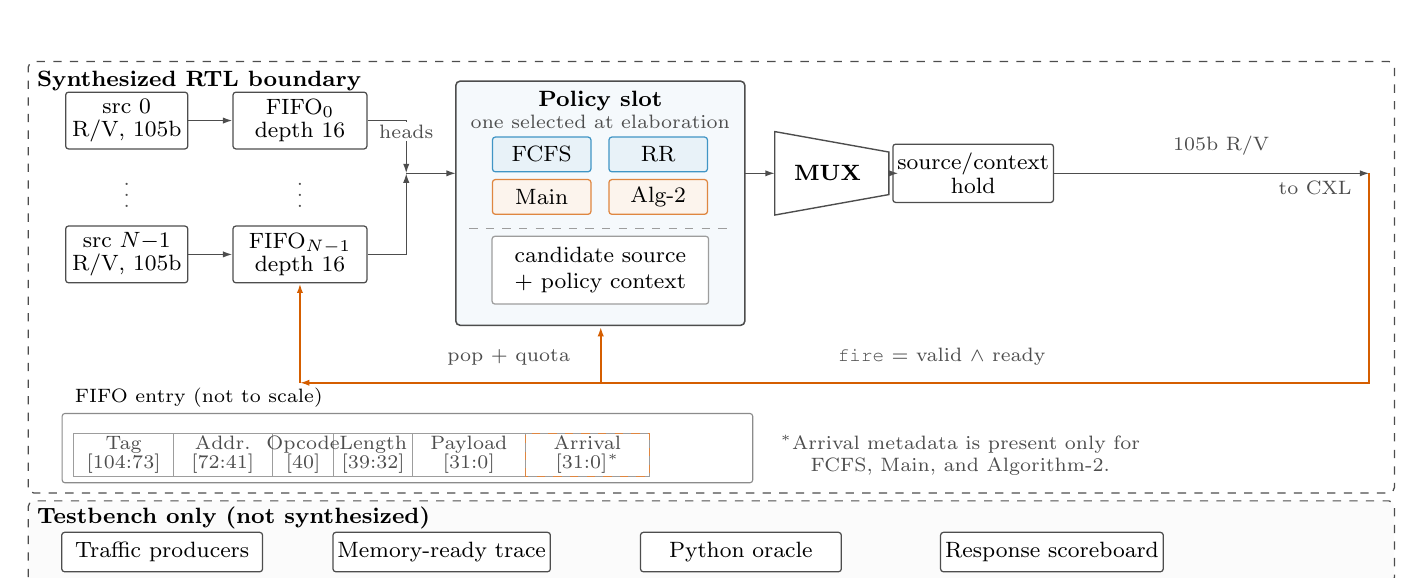
\begin{tikzpicture}[font=\footnotesize,>=Latex,
  block/.style={draw=figgray,line width=.45pt,rounded corners=1pt,fill=white,align=center,inner sep=1.6pt},
  data/.style={-{Latex[length=1.2mm,width=.8mm]},draw=figgray,line width=.5pt},
  feedback/.style={-{Latex[length=1.2mm,width=.8mm]},draw=figred,line width=.65pt},
  note/.style={font=\scriptsize,text=figgray,align=center}]
  % Synthesized boundary
  \draw[dashed,figgray,line width=.45pt,rounded corners=2pt] (-.25,1.22) rectangle (17.10,6.70);
  \node[anchor=north west,fill=white,inner sep=1pt,font=\footnotesize\bfseries]
    at (-.18,6.62) {Synthesized RTL boundary};

  % Ingress lanes and per-source FIFOs
  \node[block,minimum width=1.55cm,minimum height=.72cm] (s0) at (1.00,5.95)
    {src 0\\[-1pt]R/V, 105b};
  \node[note] at (1.00,5.10) {$\vdots$};
  \node[block,minimum width=1.55cm,minimum height=.72cm] (sn) at (1.00,4.25)
    {src $N{-}1$\\[-1pt]R/V, 105b};
  \node[block,minimum width=1.70cm,minimum height=.72cm] (f0) at (3.20,5.95)
    {FIFO$_0$\\[-1pt]depth 16};
  \node[note] at (3.20,5.10) {$\vdots$};
  \node[block,minimum width=1.70cm,minimum height=.72cm] (fn) at (3.20,4.25)
    {FIFO$_{N-1}$\\[-1pt]depth 16};
  \draw[data] (s0) -- (f0);
  \draw[data] (sn) -- (fn);

  % FIFO-head candidate bus
  \draw[data] (f0.east) -- (4.55,5.95) -- (4.55,5.28);
  \draw[data] (fn.east) -- (4.55,4.25) -- (4.55,5.28);
  \draw[data] (4.55,5.28) -- (5.18,5.28);
  \node[note,fill=white,inner sep=1pt,anchor=south] at (4.55,5.68) {heads};

  % One elaboration-time policy slot plus its retained context
  \draw[draw=figgray,line width=.55pt,rounded corners=1.5pt,fill=figblue!4]
    (5.18,3.35) rectangle (8.85,6.45);
  \node[font=\footnotesize\bfseries] at (7.015,6.20) {Policy slot};
  \node[note] at (7.015,5.93) {one selected at elaboration};
  \node[block,draw=figblue!75,fill=figblue!9,minimum width=1.25cm,minimum height=.44cm,inner sep=1pt]
    at (6.27,5.52) {FCFS};
  \node[block,draw=figblue!75,fill=figblue!9,minimum width=1.25cm,minimum height=.44cm,inner sep=1pt]
    at (7.75,5.52) {RR};
  \node[block,draw=figred!75,fill=figred!7,minimum width=1.25cm,minimum height=.44cm,inner sep=1pt]
    at (6.27,4.98) {Main};
  \node[block,draw=figred!75,fill=figred!7,minimum width=1.25cm,minimum height=.44cm,inner sep=1pt]
    at (7.75,4.98) {Alg-2};
  \draw[figgray!55,dashed,line width=.4pt] (5.35,4.58) -- (8.68,4.58);
  \node[block,draw=figgray!55,fill=white,minimum width=2.75cm,minimum height=.86cm,inner sep=1pt]
    at (7.015,4.05) {candidate source\\+ policy context};

  % Common datapath and output
  \draw[data] (8.85,5.28) -- (9.23,5.28);
  \draw[draw=figgray,line width=.5pt,fill=white]
    (9.23,4.75) -- (9.23,5.81) -- (10.68,5.55) -- (10.68,5.01) -- cycle;
  \node[font=\footnotesize\bfseries] at (9.90,5.28) {MUX};
  \node[block,minimum width=1.85cm,minimum height=.74cm] (hold) at (11.75,5.28)
    {source/context\\[-1pt]hold};
  \draw[data] (10.68,5.28) -- (10.80,5.28);
  \draw[data] (hold.east) -- (16.78,5.28);
  \node[note,above] at (14.90,5.38) {105b R/V};
  \node[note,anchor=east] at (16.68,5.10) {to CXL};

  % Fire controls FIFO pop, quota use, and held context.
  \draw[feedback] (16.78,5.28) -- (16.78,2.62) -- (3.20,2.62);
  \draw[feedback] (3.20,2.62) -- (3.20,3.88);
  \draw[feedback] (7.02,2.62) -- (7.02,3.33);
  \node[note,fill=white,inner sep=2pt,anchor=south] at (11.35,2.77)
    {\code{fire} = valid $\land$ ready};
  \node[note,fill=white,inner sep=2pt,anchor=south] at (5.85,2.77)
    {pop + quota};

  % Descriptor layout is called out separately; it is not to scale.
  \draw[draw=figgray!65,line width=.4pt,rounded corners=1pt,fill=white]
    (0.18,1.35) rectangle (8.95,2.23);
  \node[anchor=south west,font=\scriptsize,fill=white,inner sep=1pt]
    at (.30,2.26) {FIFO entry (not to scale)};
  \foreach \x/\w in {.33/1.26,1.59/1.26,2.85/.78,3.63/1.00,4.63/1.43,6.06/1.58}
    \draw[figgray!55,line width=.35pt] (\x,1.43) rectangle ++(\w,.55);
  \node[note] at (.96,1.705) {Tag\\[-1pt][104:73]};
  \node[note] at (2.22,1.705) {Addr.\\[-1pt][72:41]};
  \node[note] at (3.24,1.705) {Opcode\\[-1pt][40]};
  \node[note] at (4.13,1.705) {Length\\[-1pt][39:32]};
  \node[note] at (5.345,1.705) {Payload\\[-1pt][31:0]};
  \draw[dashed,figred!75,line width=.45pt] (6.06,1.43) rectangle (7.64,1.98);
  \node[note] at (6.85,1.705) {Arrival\\[-1pt][31:0]$^{*}$};
  \node[note,anchor=west] at (9.18,1.70)
    {$^{*}$Arrival metadata is present only for\\FCFS, Main, and Algorithm-2.};

  % Non-synthesized testbench
  \draw[dashed,figgray,line width=.45pt,rounded corners=2pt,fill=figgray!2]
    (-.25,.08) rectangle (17.10,1.12);
  \node[anchor=north west,fill=figgray!2,inner sep=1pt,font=\footnotesize\bfseries]
    at (-.18,1.08) {Testbench only (not synthesized)};
  \node[block,minimum width=2.55cm,minimum height=.50cm] at (1.45,.47) {Traffic producers};
  \node[block,minimum width=2.65cm,minimum height=.50cm] at (5.00,.47) {Memory-ready trace};
  \node[block,minimum width=2.55cm,minimum height=.50cm] at (8.80,.47) {Python oracle};
  \node[block,minimum width=2.75cm,minimum height=.50cm] at (12.75,.47) {Response scoreboard};
\end{tikzpicture}
}
\caption{Controlled synthesis boundary. The selected policy proposes a source independently of downstream readiness. The orange path denotes \code{fire}; it pops the selected FIFO, consumes service quota, and preserves the source/context hold through a stall. The testbench drives and observes DUT pins; its Python oracle is an independent reference model, and the scoreboard checks observed responses. These blocks are not synthesized.}
\label{fig:architecture}
\end{figure*}


A push is accepted when beginning-of-cycle FIFO occupancy is below 16.
The policy selects an eligible source independently of sink readiness, and
\begin{equation}
 f(t)=v_{\rm out}(t)\land r_{\rm out}(t)
 \label{eq:fire}
\end{equation}
defines successful service. Only $f(t)$ pops a FIFO and charges quota. The common
controller holds the selected source, descriptor, and policy context across a
downstream stall. Per-source ordering, admission rules, and output holding are
identical across policies.

\subsection{Capacity Is Shared; Waiting Is Scheduled}
For one equal-cost output, the measured service rate satisfies
\begin{equation}
 R=\frac{1}{T}\sum_{t=0}^{T-1}f(t)\leq 1.
 \label{eq:capacity}
\end{equation}
When the sink is ready and eligible work is continuously available, a
work-conserving implementation attains $R=1$. Changing the arbiter can then
change the order of service, source shares, and latency distributions while
leaving aggregate capacity fixed. This is the theoretical basis for evaluating
sparse tails alongside throughput: equal throughput does not imply equal
quality of service.

FCFS chooses the oldest admitted head, with source-ID tie breaking. Sparse
requests therefore compete with older requests already admitted from the heavy
source. Depth-16 FIFOs constrain this admitted competition, while unaccepted
heavy requests remain in the producer queue. RR10 instead rotates across
nonempty sources, granting up to ten successful transfers per visit and skipping
empty sources. It organizes competition by source identity rather than arrival
age. Sink stalls consume no quantum under either quota-based policy.

\subsection{Classification Changes the Service Domain}
Main measures successful transfers $B[h]$ for each source in a $W$-cycle window,
with $S=\sum_h B[h]$. Its threshold evidence is
\begin{align}
 \mathrm{UP}:&\quad 10NB[h]<3S,\nonumber\\
 \mathrm{DOWN}:&\quad NB[h]>S,\label{eq:classes}\\
 \mathrm{KEEP}:&\quad \text{otherwise, including equality}.\nonumber
\end{align}
Production uses $W=5{,}000{,}000$, 23-bit counters, and widened unsigned 32-bit
comparisons. The closing transfer is included before counters clear. Every
source starts effective High. Two supporting windows commit a transition;
a pending state retains its previous effective class. KEEP, opposite evidence,
or an idle window cancels the pending transition. Thus classification reflects
delivered service over time rather than a transient arrival spike.

Main alternates visits to High and Low, each with a quota of up to ten fires,
and selects the oldest head within the active class. In the heavy/sparse case,
two windows move the heavy source to Low while sparse sources remain High.
Older heavy entries then compete in a different service domain from sparse
entries. A sparse request still waits for applicable visit context, but its
priority no longer depends on outranking every heavy head by age.

An empty High visit immediately relinquishes unused quota. That credit is not
banked, and Low proceeds without an artificial idle slot. The 10/10 schedule
therefore divides visits when both classes need service; it does not reserve
half the output for absent sparse work. This rule explains how Main preserves
full output service while the heavy host uses approximately 97.7\% of it.

Class aggregation also predicts a burst trade-off. Several sparse sources
share one ten-fire High visit, whereas RR10 assigns ten fires to each source.
Overlapping sparse bursts can exhaust the shared High visit and wait through
Low service. This structural explanation is consistent with the observed
burst tails and motivates reporting Main versus RR10 separately from Main
versus FCFS.

\section{Implementation and Experimental Method}
\subsection{Correctness and Comparable Hardware}
One policy-selectable SystemVerilog top shares FIFO, mux, and hold logic.
Independent Python queue models and cocotb compare output pins, descriptors,
source order, conservation, response tags, occupancy, and held-output stability.
Directed tests exercise timestamp wrap, full-plus-pop refusal, no bypass, quota
boundaries, class thresholds, and reset during output holding. The accepted
primary regression contains 180/180 runs across three policies, three source
counts, and 20 seeds. Main additionally passes 30 stress runs and three
20-million-cycle production runs across $N=4,8,16$.

Formality W-2024.09 verifies 14/14 scoped RTL/netlist pairs: nine primary
mappings, two supplementary mappings, and three current-Main bridges. The pairs
have zero failing, aborted, unverified, unmatched, or active-blackbox points.
An intentional output-valid inversion fails its expected compare point,
providing a negative control. Six FCFS/RR pairs retain one explicitly
uncompared propagated-constant register. The supplementary Algorithm-2 study
passes ten stress cases and a production run; at $N=4$ its complete-area
difference from Main is 0.028626\%. We retain it as transition-semantic
sensitivity evidence and focus the primary comparison on FCFS, RR10, and Main.

The nine primary area/timing mappings use Design Compiler and PrimeTime
W-2024.09, SAED32 RVT at TT, 0.78\,V and $25\,{}^\circ$C. The common clock is
25\,ns, setup/hold uncertainty is 0.10/0.05\,ns, input/output delays are
0/2\,ns, and the nominal output load is 2.656828\,fF. A common wire-load
estimate and identical constraints define the pre-layout comparison. Final
checks restore the original output capacitance limits after optimization.
Area is reported in library units. The accepted cold-power matrix uses
zero-delay VCS mapped-netlist replay and switching activity interchange format
(SAIF) data in PrimeTime/PrimePower
at the same corner and clock, covering three seeds per mapping.

\subsection{Production HOG-SPARSE Experiment}
The accepted HOG-SPARSE experiment contains $3\times5=15$ actual RTL runs at
$N=4$, depth 16, with seeds 509--513 and a continuously ready sink. Source zero
generates one descriptor per active cycle. Sources one through three have
low demand, driven by deterministic policy-independent random streams.
Each run executes ten million real training cycles, covering two complete
production windows. Main's heavy source follows High, pending High, then Low;
the sparse sources remain effective High. The measured class map is
Low/High/High/High.

Profile A continues independent Bernoulli arrivals with probability $1/128$
per sparse source per cycle for 100,000 measured cycles. Profile B generates
one eight-descriptor burst per sparse source per 1,024-cycle block, at a seeded
uniform offset, for 102,400 cycles. Its 100 blocks generate exactly 2,400 sparse
requests. Both profiles have expected sparse demand $3/128$ requests/cycle;
A retains its realized finite counts. The heavy source supplies persistent
competition throughout training, both profiles, and completion guards.

Each profile is followed by a 1,024-cycle guard that stops new sparse arrivals
while maintaining heavy generation. Every sparse cohort completes with heavy
pressure still active. Final drain then completes all producer, FIFO, and
response work. The accepted execution accounts for 156,657,531 nonreset RTL
cycles, including 150 million training cycles and 3,036,000 measured cycles.
All 15 production runs pass, and an independent raw audit passes. The audit
checks exact histograms, source pooling, direct/stage identities, conservation,
class transitions, completion, and actual run exits. Five external trace groups
match across policies; Main and FCFS also have identical cold pin digests over
each seed's entire ten-million-cycle training interval.

\subsection{Endpoints and Paired Summaries}
For request $i$, generation, acceptance, and fire cycles are $g_i,a_i,d_i$.
The primary endpoint is direct sparse latency
\begin{equation}
 L_i=d_i-g_i=(a_i-g_i)+(d_i-a_i).
 \label{eq:latency}
\end{equation}
Each run pools the complete sparse generation cohort of one profile and takes
nearest-rank P99 directly from its request histogram. Per-source results remain
available for checking distribution within the class. Figures report arithmetic
means of five run means or five run P99s; whiskers denote observed seed ranges.
For baseline $b$ and matched seed $s$, the percentage reduction is
\begin{equation}
 \rho_{b,s}=100\frac{P99_{b,s}-P99_{{\rm Main},s}}{P99_{b,s}}.
 \label{eq:paired}
\end{equation}
We average these five paired percentages. This preserves the matched comparison
and differs from taking a ratio of two mean P99s. Five seeds are descriptive
replications; the three sparse sources within a run share the same arbiter.

\section{Evaluation}
\subsection{Sparse Protection at Full Output Capacity}
Figure~\ref{fig:hog-sparse} connects sparse waiting to heavy service. In profile A,
FCFS has mean direct latency \HSMeanAFCFS\ cycles and mean run P99
\HSPtailAFCFS\ cycles. Main reduces these to \HSMeanAMain\ and
\HSPtailAMain\ cycles. The P99 reduction averages 8.2 cycles and
\HSReductionAFCFS\% across matched seeds, with five of five improving. RR10
achieves \HSMeanARR\ cycles mean and \HSPtailARR\ cycles P99. Main's one-cycle
P99 advantage over RR10 is \HSReductionARR\%, again in all five seeds.

\begin{figure*}[t]
\centering
\begin{tikzpicture}
\begin{groupplot}[
  group style={group size=2 by 2,horizontal sep=5.5em,vertical sep=4.8em},
  width=.435\textwidth,height=3.65cm,
  title style={font=\small},tick label style={font=\footnotesize,text=figgray},
  label style={font=\footnotesize},
  axis line style={figgray!70},tick style={figgray!70},
  axis x line=bottom,axis y line=left,
  ymajorgrids,grid style={figgray!18,line width=.25pt},
  xmin=.55,xmax=2.45,xtick={1,2},xticklabels={A: single arrivals,B: eight-request bursts},
  xlabel={Sparse arrival profile},
  /pgfplots/error bars/y dir=both,/pgfplots/error bars/y explicit,
  /pgfplots/error bars/error bar style={line width=.6pt},
  /pgfplots/error bars/error mark options={mark size=2pt}]
\nextgroupplot[title={(a) Sparse mean latency},ylabel={Generation-to-fire (cycles)},
  ymin=0,ymax=28,ytick={0,5,10,15,20,25},ybar,bar width=10pt]
\addplot[fill=figblue!65,draw=figblue,bar shift=-11pt] table[x=x,y=y,y error minus=lo,y error plus=hi]{\HSMeanFCFS};
\addplot[fill=figgray!25,draw=figgray,dashed,bar shift=0pt] table[x=x,y=y,y error minus=lo,y error plus=hi]{\HSMeanRR};
\addplot[fill=figred!65,draw=figred,bar shift=11pt] table[x=x,y=y,y error minus=lo,y error plus=hi]{\HSMeanMain};
\nextgroupplot[title={(b) Sparse P99 latency},ylabel={Generation-to-fire P99 (cycles)},
  ymin=0,ymax=40,ytick={0,10,20,30,40},ybar,bar width=10pt]
\addplot[fill=figblue!65,draw=figblue,bar shift=-11pt] table[x=x,y=y,y error minus=lo,y error plus=hi]{\HSPtailFCFS};
\addplot[fill=figgray!25,draw=figgray,dashed,bar shift=0pt] table[x=x,y=y,y error minus=lo,y error plus=hi]{\HSPtailRR};
\addplot[fill=figred!65,draw=figred,bar shift=11pt] table[x=x,y=y,y error minus=lo,y error plus=hi]{\HSPtailMain};
\nextgroupplot[title={(c) Main's paired P99 change},ylabel={P99 reduction (\%)},
  xmin=.5,xmax=4.5,xtick={1,2,3,4},xticklabels={A/FCFS,A/RR10,B/FCFS,B/RR10},
  xlabel={Profile / comparison baseline},ymin=-50,ymax=60,ytick={-40,-20,0,20,40,60}]
\addplot[figgray,densely dashed,no marks,forget plot] coordinates {(.5,0)(4.5,0)};
\addplot[only marks,figgray,mark=*,mark size=1.15pt,forget plot] coordinates {\HSPairedSeeds};
\addplot[only marks,figred,mark=diamond*,mark size=3pt] table[x=x,y=y,y error minus=lo,y error plus=hi]{\HSPaired};
\nextgroupplot[title={(d) Heavy service at full capacity},ylabel={Transfers / measured cycle},
  ymin=0,ymax=1.12,ytick={0,.25,.5,.75,1},ybar,bar width=10pt]
\addplot[fill=figblue!65,draw=figblue,bar shift=-11pt] table[x=x,y=y,y error minus=lo,y error plus=hi]{\HSHeavyFCFS};
\addplot[fill=figgray!25,draw=figgray,dashed,bar shift=0pt] table[x=x,y=y,y error minus=lo,y error plus=hi]{\HSHeavyRR};
\addplot[fill=figred!65,draw=figred,bar shift=11pt] table[x=x,y=y,y error minus=lo,y error plus=hi]{\HSHeavyMain};
\addplot[black,densely dashed,line width=.7pt,no marks,sharp plot,forget plot] coordinates {(.55,1)(2.45,1)};
\end{groupplot}
\node[anchor=south,font=\footnotesize,yshift=31pt] at
  ($(group c1r1.north west)!.5!(group c2r1.north east)$)
  {\tikz\draw[fill=figblue!65,draw=figblue] (0,0) rectangle (.22,.12);\ FCFS\qquad
   \tikz\draw[fill=figgray!25,draw=figgray,dashed] (0,0) rectangle (.22,.12);\ RR10\qquad
   \tikz\draw[fill=figred!65,draw=figred] (0,0) rectangle (.22,.12);\ Main};
\end{tikzpicture}
\caption{\textbf{Sparse-host protection with unchanged output capacity.}
Fifteen production RTL runs, $N=4$, seeds 509--513, two real $W=5$M training windows per run.
(a,b) Bars are equal-weight means of five run means and five run P99s, respectively;
whiskers span the observed seed minimum and maximum, not confidence intervals.
(c) Diamonds are mean paired percentage reductions; dots are the five matched seeds
(horizontal jitter is for visibility). Positive values favor Main.
(d) Bars show heavy-host service; the dashed line is total output service,
exactly 1.000000 transfer/cycle in every measured interval. Heavy share remains
97.66--97.67\%; its seed ranges are smaller than the plotting resolution.
Profile A lasts 100,000 cycles; B lasts 102,400 cycles.}
\label{fig:hog-sparse}
\end{figure*}


Profile B preserves Main's advantage over FCFS under burst injection. FCFS
reaches \HSMeanBFCFS\ cycles mean and \HSPtailBFCFS\ cycles P99; Main reaches
\HSMeanBMain\ and \HSPtailBMain\ cycles. The paired reduction is 13.0 cycles
or \HSReductionBFCFS\%, with all five seeds improving. Across the three sparse
sources and five seeds, every one of the 15 source/seed P99 comparisons improves
over FCFS in each profile. The aggregate result therefore corresponds to
protection across the sparse hosts in this experiment.

The stage measurements locate the benefit. Profile A's generation-to-acceptance
mean is zero for every policy: sparse requests enter their own FIFOs immediately.
The reduction occurs during arbitration after admission. In B, all policies
incur the same 3.5-cycle mean injection delay because eight descriptors generated
together enter a source FIFO at one per cycle. Main's acceptance-to-fire mean is
5.8243 cycles, versus FCFS's 19.7989. The direct endpoint includes this common
injection cost and measures each request's full wait; it is not constructed by
adding stage percentiles.

The cold control reinforces the interpretation. Before the second classification
takes effect, Main and FCFS have matching per-seed sparse histograms, a
five-run mean of 16.3842 cycles, and P99 of 18 cycles. Their full training pin
digests match as well. Main begins with the FCFS service domain and obtains
sparse protection after the intended class separation becomes effective.
The controlled comparisons remain between policies under matched arrivals at
each phase.

\subsection{The RR10 Burst Trade-off}
RR10's profile-B mean is \HSMeanBRR\ cycles, close to Main's \HSMeanBMain,
but its mean run P99 is \HSPtailBRR\ cycles versus Main's \HSPtailBMain.
Main's paired P99 reduction relative to RR10 is negative: $-20.78\%$, or
$-3.6$ cycles. Four seeds have a higher Main P99 and one ties. Main's run P99s
span 17--24 cycles, while RR10 spans 17--18. Similar means thus coexist with
different upper tails.

These results fit the service domains in Section~3. Single sparse requests
benefit from bypassing heavy arrival age through the High class. When several
sparse bursts overlap, they compete within one shared High visit; RR10 retains
a separate quantum per source. Class aggregation is therefore a plausible
mechanistic explanation for the measured burst-tail difference. The policy
choice depends on whether the target traffic values sparse single-arrival
protection or tighter burst tails under this source mix.

\subsection{Heavy Service and Conservation}
All 30 measured policy/seed/profile intervals sustain exactly 1.000000
transfer/cycle with zero avoidable eligible-ready bubbles. In A, heavy
transfers/cycle average 0.976728 for FCFS, 0.976726 for RR10, and 0.976724
for Main. In B, the respective rates are 0.97657617, 0.97656445, and
0.97656445. Because total service is one, these rates are also the heavy
host's service fractions: approximately 97.66--97.67\%.

Main's mean heavy-rate difference from FCFS in A is only $-0.000004$
transfer/cycle. Empty-High relinquishment lets the heavy Low source consume
spare opportunities, so sparse protection does not impose a 50\% heavy-host
cap. The small interval differences include requests crossing phase boundaries;
the complete-cohort latency and final conservation checks retain those requests.

Total offered load exceeds capacity because the heavy host alone offers one
request per cycle. Its producer backlog grows under every policy; at B-end,
mean pending counts are 239,330.4 for FCFS and 239,331.6 for RR10 and Main.
These counts describe unaccepted producer work, separate from each depth-16
FIFO. Complete final drain accounts for every generated heavy request, while
the sparse completion guards establish protection during continuing interference.

\subsection{Policy-to-Hardware Cost}
Figure~\ref{fig:hardware-cost} places the service result beside the accepted
hardware comparison. All nine primary mappings meet setup, hold, and original
electrical limits at the common 25\,ns target. Main adds 5.89\%, 5.23\%, and
4.97\% total area over FCFS at $N=4,8,16$, respectively. Its premiums over
RR10 are 39.27\%, 38.60\%, and 38.22\%. At the four-source boundary used
for HOG-SPARSE, Main's area is 110,089.846 library units, compared with
103,970.058 for FCFS and 79,047.172 for RR10. The measured sparse-host
protection over FCFS therefore accompanies a 5.89\% complete-area premium
at the same source count.

\begin{figure*}[t]
\centering
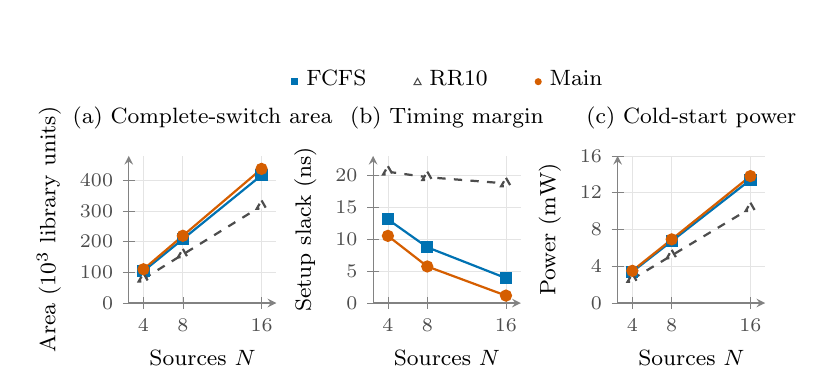
\begin{tikzpicture}
\begin{groupplot}[
  group style={group size=3 by 1,horizontal sep=3.5em},
  width=.285\textwidth,height=3.45cm,
  title style={font=\footnotesize},tick label style={font=\scriptsize,text=figgray},
  label style={font=\footnotesize},axis line style={figgray!70},tick style={figgray!70},
  grid=major,grid style={figgray!15,line width=.25pt},
  axis x line=bottom,axis y line=left,
  xmin=2.5,xmax=17.5,xtick={4,8,16},xlabel={Sources $N$}]
\nextgroupplot[title={(a) Complete-switch area},ylabel={Area ($10^3$ library units)},
  ymin=0,ymax=480,ytick={0,100,200,300,400}]
\addplot[figblue,line width=.8pt,mark=square*,mark size=1.8pt] coordinates {\AreaFCFS};
\addplot[figgray,line width=.8pt,dashed,mark=triangle*,mark options={fill=white},mark size=2pt] coordinates {\AreaRR};
\addplot[figred,line width=.8pt,mark=*,mark size=1.8pt] coordinates {\AreaMain};
\nextgroupplot[title={(b) Timing margin},ylabel={Setup slack (ns)},
  ymin=0,ymax=23,ytick={0,5,10,15,20}]
\addplot[figblue,line width=.8pt,mark=square*,mark size=1.8pt] coordinates {\SetupFCFS};
\addplot[figgray,line width=.8pt,dashed,mark=triangle*,mark options={fill=white},mark size=2pt] coordinates {\SetupRR};
\addplot[figred,line width=.8pt,mark=*,mark size=1.8pt] coordinates {\SetupMain};
\nextgroupplot[title={(c) Cold-start power},ylabel={Power (mW)},
  ymin=0,ymax=16,ytick={0,4,8,12,16}]
\addplot[figblue,line width=.8pt,mark=square*,mark size=1.8pt] coordinates {\ColdMeanFCFS};
\addplot[figgray,line width=.8pt,dashed,mark=triangle*,mark options={fill=white},mark size=2pt] coordinates {\ColdMeanRR};
\addplot[figred,line width=.8pt,mark=*,mark size=1.8pt] coordinates {\ColdMeanMain};
\end{groupplot}
\node[anchor=south,font=\footnotesize,yshift=22pt] at
  ($(group c1r1.north west)!.5!(group c3r1.north east)$)
  {\tikz\fill[figblue] (0,0) rectangle (.09,.09);\ FCFS\qquad
   \tikz\draw[figgray] (0,0)--(.045,.08)--(.09,0)--cycle;\ RR10\qquad
   \tikz\fill[figred] (0,0) circle (.045);\ Main};
\end{tikzpicture}
\caption{\textbf{The hardware price of service differentiation.}
Accepted SAED32 RVT mappings at TT, 0.78\,V, $25\,{}^\circ$C and a common 25\,ns clock.
(a,b) One mapped observation per policy and $N$; lines connect measured points.
(c) Means of three accepted cold-start seed estimates; seed variation is below
the marker size at this scale. At $N=16$, the tool prints power to 0.1\,mW.
Power is a separate zero-delay mapped-netlist activity experiment; the
HOG-SPARSE latency experiment contributes no new power estimate.
Each panel has its own labeled axes and units.}
\label{fig:hardware-cost}
\end{figure*}


FIFO subtrees account for 92.40--98.63\% of complete mapped area, including
arrival metadata where required. At $N=16$, 256 FIFO entries hold 26,880
descriptor bits; FCFS and Main add 8,192 arrival bits. RR10's smaller
storage footprint is a real consequence of its service rule. Main further
adds window counters, class state, and quota context. Its policy subtree
grows from 7,143.988 library units at $N=4$ to 26,673.175 at $N=16$,
whereas FCFS grows from 1,131.957 to 6,038.461 and RR10 from 263.039
to 1,268.687. These subtree values isolate logic organization; the
complete-area comparison also charges the ordering metadata in the FIFOs.

Timing follows the same increase in selection and classification work.
FCFS setup slack decreases from 13.072\,ns at $N=4$ to 3.892\,ns at
$N=16$; Main decreases from 10.496 to 1.158\,ns. RR10 retains at least
18.694\,ns. Main16's limiting path connects FIFO read-pointer state to
class-state update, linking head selection to the closing-window decision.
All reported designs use the common pipeline and constraints. The accepted
timing accounting retains 140 constant-disabled checks separately, so closure
refers to evaluated setup, hold, and electrical checks under this profile.

Cold-start power consistently orders RR10 $<$ FCFS $<$ Main for every
accepted seed. The three-seed means at $N=4$ are approximately 2.601,
3.398, and 3.500\,mW; at $N=16$ they are 10.3, 13.4, and 13.8\,mW.
This experiment characterizes clocked storage, leakage, and switching under
its own cold activity trace. The production HOG-SPARSE experiment supplies
trained-state latency and service results, while the power estimates retain
their original activity assumptions. A separate boundary-focused replay
exercises classification at 50 times its natural event density and is
interpreted as mechanism sensitivity rather than an average power figure.

\section{Conclusion}
The RTL comparison establishes a concrete service-to-cost exchange. After
two production classification windows, Main reduces sparse P99 relative to
FCFS by 45.03\% for single arrivals and 38.64\% for bursts, with every seed
improving and full output capacity preserved. The heavy host retains
approximately 97.7\% of service because unused class quota is relinquished.
RR10 exposes the complementary design point: it is smaller and provides a
tighter burst tail, while Main slightly improves the single-arrival tail.

\newpage
The hardware result explains the price of that choice. Main's complete-area
premium over FCFS is 4.97--5.89\%, all nine mappings close at 25\,ns, and
FIFO storage dominates the mapped boundary. Arrival metadata makes RR10's
area advantage materially larger. For this switch slice, choosing an
arbitration policy means choosing a waiting distribution together with its
ordering state, classification logic, and storage cost. Reporting those
quantities at a common boundary turns an abstract fairness mechanism into
an assessable hardware design decision.

\section{AI Use Acknowledgment}
Claude Code/RTL Agent Team and owner-authorized GPT-6.1 Sol supported implementation
and verification tooling; Codex coordinated evidence review and drafted this
version using ARS-Codex guidance. Earlier Gemini 3.8 Flash and Gemini 4 Argon
assisted literature reading and claim review. A Gemini 3.8 Flash language-polish
pass is planned after this draft. Prompts and responses are retained; numerical
claims derive from archived tool results. The authors take responsibility for
the report and its sources.

\clearpage

\begingroup\footnotesize
\begin{thebibliography}{99}
\bibitem{cxl_intro} D. Das Sharma, R. Blankenship, and D. Berger, ``An Introduction to the Compute Express Link (CXL) Interconnect,'' \emph{ACM Computing Surveys}, vol.~56, no.~11, pp.~1--37, 2024. doi: \href{https://doi.org/10.1145/3669900}{10.1145/3669900}.
\bibitem{pond} H. Li \emph{et al.}, ``Pond: CXL-Based Memory Pooling Systems for Cloud Platforms,'' in \emph{Proc. 28th ACM Int. Conf. Architectural Support for Programming Languages and Operating Systems}, vol.~2, 2023, pp.~574--587. doi: \href{https://doi.org/10.1145/3575693.3578835}{10.1145/3575693.3578835}.
\bibitem{tpp} H. Al Maruf \emph{et al.}, ``TPP: Transparent Page Placement for CXL-Enabled Tiered-Memory,'' in \emph{Proc. 28th ACM Int. Conf. Architectural Support for Programming Languages and Operating Systems}, vol.~3, 2023, pp.~742--755. doi: \href{https://doi.org/10.1145/3582016.3582063}{10.1145/3582016.3582063}.
\bibitem{directcxl} D. Gouk, M. Kwon, H. Bae, S. Lee, and M. Jung, ``Memory Pooling With CXL,'' \emph{IEEE Micro}, vol.~43, no.~2, pp.~48--57, 2023. doi: \href{https://doi.org/10.1109/MM.2023.3237491}{10.1109/MM.2023.3237491}.
\bibitem{case_pool} P. Levis, K. Lin, and A. Tai, ``A Case Against CXL Memory Pooling,'' in \emph{Proc. 22nd ACM Workshop on Hot Topics in Networks}, 2023, pp.~18--24. doi: \href{https://doi.org/10.1145/3626111.3628195}{10.1145/3626111.3628195}.
\bibitem{my_cxl_pool} Y. Zhong \emph{et al.}, ``My CXL Pool Obviates Your PCIe Switch,'' in \emph{Proc. Workshop on Hot Topics in Operating Systems}, 2025, pp.~58--66. doi: \href{https://doi.org/10.1145/3713082.3730393}{10.1145/3713082.3730393}.
\bibitem{stfm} O. Mutlu and T. Moscibroda, ``Stall-Time Fair Memory Access Scheduling for Chip Multiprocessors,'' in \emph{Proc. 40th IEEE/ACM Int. Symp. Microarchitecture}, 2007, pp.~146--160. doi: \href{https://doi.org/10.1109/MICRO.2007.21}{10.1109/MICRO.2007.21}.
\bibitem{fqmem} K. J. Nesbit, N. Aggarwal, J. Laudon, and J. E. Smith, ``Fair Queuing Memory Systems,'' in \emph{Proc. 39th IEEE/ACM Int. Symp. Microarchitecture}, 2006, pp.~208--222. doi: \href{https://doi.org/10.1109/MICRO.2006.24}{10.1109/MICRO.2006.24}.
\bibitem{atlas} Y. Kim, D. Han, O. Mutlu, and M. Harchol-Balter, ``ATLAS: A Scalable and High-Performance Scheduling Algorithm for Multiple Memory Controllers,'' in \emph{Proc. 16th IEEE Int. Symp. High-Performance Computer Architecture}, 2010, pp.~1--12. doi: \href{https://doi.org/10.1109/HPCA.2010.5416658}{10.1109/HPCA.2010.5416658}.
\bibitem{tcm} Y. Kim, M. Papamichael, O. Mutlu, and M. Harchol-Balter, ``Thread Cluster Memory Scheduling: Exploiting Differences in Memory Access Behavior,'' in \emph{Proc. 43rd IEEE/ACM Int. Symp. Microarchitecture}, 2010, pp.~65--76. doi: \href{https://doi.org/10.1109/MICRO.2010.51}{10.1109/MICRO.2010.51}.
\bibitem{bliss} L. Subramanian, D. Lee, V. Seshadri, H. Rastogi, and O. Mutlu, ``The Blacklisting Memory Scheduler: Achieving High Performance and Fairness at Low Cost,'' in \emph{Proc. IEEE 32nd Int. Conf. Computer Design}, 2014, pp.~8--15. doi: \href{https://doi.org/10.1109/ICCD.2014.6974655}{10.1109/ICCD.2014.6974655}.
\bibitem{fai} J. Li, Y. Liu, Y. Gu, and C. Wu, ``FAI-CXL: An Efficient Hardware-Accelerated Fairness-Aware CXL Memory Pool Management with Fine-Grained Cacheline-Level Interleaving,'' in \emph{Proc. IEEE Int. Conf. Parallel and Distributed Systems (ICPADS)}, 2025, pp.~1--8. doi: \href{https://doi.org/10.1109/ICPADS67057.2025.11322896}{10.1109/ICPADS67057.2025.11322896}. Algorithm 2, p.~5.
\bibitem{cxl_interplay} S. Mao \emph{et al.}, ``CXL-INTERPLAY: Unraveling and Characterizing CXL Interference in Modern Computer Systems,'' in \emph{Proc. 62nd ACM/IEEE Design Automation Conference}, 2025, pp.~1--7. doi: \href{https://doi.org/10.1109/DAC63849.2025.11132607}{10.1109/DAC63849.2025.11132607}.
\bibitem{contention_cache} C. Tirumalasetty and N. R. Annapareddy, ``Contention Aware DRAM Caching for CXL-Enabled Pooled Memory,'' in \emph{Proc. Int. Symp. Memory Systems}, 2024, pp.~157--171. doi: \href{https://doi.org/10.1145/3695794.3695808}{10.1145/3695794.3695808}.
\bibitem{hpc_pool} J. Wahlgren, M. Gokhale, and I. B. Peng, ``Evaluating Emerging CXL-Enabled Memory Pooling for HPC Systems,'' in \emph{Proc. IEEE/ACM Workshop on Memory Centric High Performance Computing}, 2022, pp.~11--20. doi: \href{https://doi.org/10.1109/MCHPC56545.2022.00007}{10.1109/MCHPC56545.2022.00007}.
\bibitem{cxldmsim} Y. Wang \emph{et al.}, ``CXL-DMSim: A Full-System CXL Disaggregated Memory Simulator With Comprehensive Silicon Validation,'' \emph{IEEE Trans. Computer-Aided Design of Integrated Circuits and Systems}, vol.~45, no.~4, pp.~1787--1801, 2026. doi: \href{https://doi.org/10.1109/TCAD.2025.3607145}{10.1109/TCAD.2025.3607145}.



\bibitem{rixner} S. Rixner, W. J. Dally, U. J. Kapasi, P. Mattson, and J. D. Owens, ``Memory Access Scheduling,'' in \emph{Proc. 27th Int. Symp. Computer Architecture}, 2000, pp.~128--138. doi: \href{https://doi.org/10.1145/339647.339668}{10.1145/339647.339668}.
\bibitem{gupta} P. Gupta and N. McKeown, ``Designing and Implementing a Fast Crossbar Scheduler,'' \emph{IEEE Micro}, vol.~19, no.~1, pp.~20--28, 1999. doi: \href{https://doi.org/10.1109/40.748793}{10.1109/40.748793}.
\bibitem{wfq_sort} K. McLaughlin, S. Sezer, H. Blume, X. Yang, F. Kupzog, and T. Noll, ``A Scalable Packet Sorting Circuit for High-Speed WFQ Packet Scheduling,'' \emph{IEEE Trans. Very Large Scale Integration (VLSI) Systems}, vol.~16, no.~7, pp.~781--791, 2008. doi: \href{https://doi.org/10.1109/TVLSI.2008.2000323}{10.1109/TVLSI.2008.2000323}.
\bibitem{arbiter_ppa} S. Singh, J. Ravindra, and B. R. Naik, ``Power and Area Calibration of Switch Arbiter for High Speed Switch Control and Scheduling in Network-on-Chip,'' in \emph{Proc. Int. SoC Design Conf.}, 2016, pp.~5--6. doi: \href{https://doi.org/10.1109/ISOCC.2016.7799765}{10.1109/ISOCC.2016.7799765}.
\bibitem{artifact} J. Chiang and D. Chou, \emph{CXL Scheduler Project: Frozen Specification v1.0 and Experimental Evidence}, ECE 509 project artifact, 2026. Specification commit \code{1af80967}; PPA evidence snapshot \code{9141dfe}; accepted HOG-SPARSE run \code{20261022T034507Z\_311}. Source manifests and reproduction instructions accompany this report.
\end{thebibliography}
\endgroup
\end{document}
